% !TeX spellcheck = en_US

\chapter{Analysis}
The Analysis shows use-cases for the system based on the stakeholders. A gap-analysis is performed to compare use-cases of the new system in difference to the old one. The result of this process will be requirements, which are separated into functional and non-functional.


\section{Stakeholders}
Stakeholders are groups of people that have an interest in the system. This can be from a practical, or from a business standpoint. 

\subsection{Model Developer}
The Model Developer is a technical user that creates a MARS model in cooperation with a domain expert.

\subsection{Simulation Developer}
The Model Developer is an domain export. He Uses the Model, created by the Model Developer to answer a research question.

\subsection{Group Admin}
The Group Admin is a user of the system with a leading roll in his group. He wants to manage people belonging to a particular group and handle group dependent settings.

\subsection{Admin}
The Admin is a global acting user with far reaching permission inside the system.


\section{Use-cases}
The interaction with the system requires 7 main use-cases. These cases are following the central workflow, while 2 extra use-cases are for management purposes. Figure \ref{fig:use-cases} shows an overview.\\
This piece of work focuses on the highlighted area of the use-cases, which are described in the following paragraphs.
\begin{figure}[H]
	\centering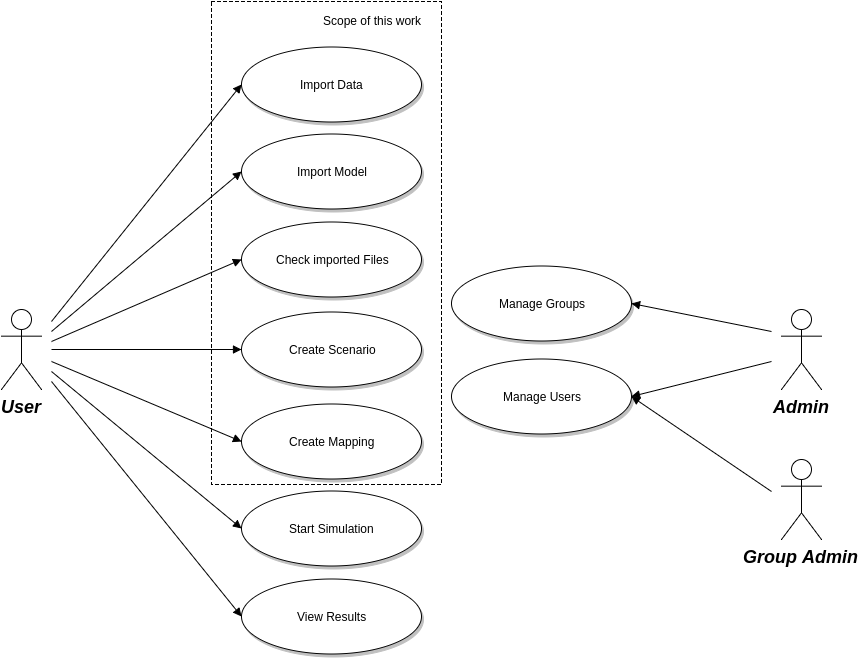
\includegraphics[width=1\textwidth]{res/Use-Cases}
	\caption{Use-Cases in UML notation}
	\label{fig:use-cases}
\end{figure}

\subsection{Import Data}

\subsection{Import Model}

\subsection{Check imported Data}

\subsection{Create Mapping}



\section{Gap-Analysis}


\section{Requirements}

\subsection{Functional Requirements}

\subsection{Non-Functional Requirements}
